%For arxiv submission
\documentclass[useAMS, usenatbib]{mnras}
\usepackage{graphicx,amsmath,color,amssymb}
%\voffset=-0.8in
%MNRAS
%\documentclass[useAMS, usenatbib, usegraphicx, twocolumn]{mnras}

\usepackage[pdftitle={A hybrid particle-analytic method for non-linear neutrino structure}, draft]{hyperref}
% \newcommand{\eprint}[1]{\href{http://arxiv.org/abs/#1}{#1}}
% \newcommand{\adsurl}[1]{\href{#1}{ADS}}

\topmargin -1.5cm
\bibliographystyle{mnras}

\newcommand{\beq}{\begin{equation}}
\newcommand{\eeq}{\end{equation}}
\newcommand{\barr}{\begin{eqnarray}}
\newcommand{\earr}{\end{eqnarray}}

\newcommand{\rme}{\textrm{e}}
\newcommand{\rmH}{\textrm{H}}
\newcommand{\Ly}{\textrm{Ly}}
\newcommand{\pabn}{p_{\textrm{ab}}^n}
\newcommand{\pscn}{p_{\textrm{sc}}^n}
\newcommand{\rmd}{\textrm{d}}
\newcommand{\N}{\mathcal{N}}
\newcommand{\nuc}{\nu_{\rm c}}
\newcommand{\Tm}{T_{\rm m}}
\newcommand{\Tr}{T_{\rm r}}
\newcommand{\nh}{n_{\rm H}}
\newcommand{\bfA}{\boldsymbol{A}}
\newcommand{\bfr}{\boldsymbol{r}}
\newcommand{\bfV}{\boldsymbol{V}}
\newcommand{\bs}{\mathbf}
\newcommand{\mH}{\mathcal{H}}

\newcommand{\natu}{Nature (London)}
\newcommand{\aas}{Bull. Am. Astron. Soc.}
\newcommand{\gadget}{{\small GADGET\,}}

\newcommand{\spb}[1]{{\textsc{\textcolor{red}{[{\bf SPB}: #1]}}}}
\newcommand{\yah}[1]{{\textcolor{blue}{[{\bf YAH}: #1]}}}



\newcommand{\Mpch}{\,\mathrm{Mpc} \,h^{-1}}
\newcommand{\hMpc}{h^{-1}\,\mathrm{Mpc}}
\newcommand{\Lya}{Lyman-$\alpha\;$}
%%%%%%%%%%%%%%%%%%%%%%%%%%%%%%%%%%%%%%%%%%%%%%%%%%%%%%%%%%%%%%%%%%%%%%%%%%%%%%%%%%%%%%%%%%%%%%%%%%


\title{A Hybrid Method for Simulating Non-Linear Neutrino Structure}
\author[ S. Bird et al.]{  Simeon Bird\thanks{E-mail: sbird@ucr.edu}, Yacine Ali-Ha\"{\i}moud, Yu Feng, Jia Liu\vspace{1.5mm}\\
No longer at Institute for Advanced Study, Einstein Drive, Princeton, New Jersey 08540}

\begin{document}

\date{\today}

\pagerange{\pageref{firstpage}--\pageref{lastpage}} \pubyear{2012}
\pagenumbering{arabic}
\label{firstpage}

\maketitle

\begin{abstract}
\end{abstract}

\begin{keywords}
        neutrinos - cosmology: large-scale structure of Universe - cosmology: dark matter
\end{keywords}

\section{Introduction}

%Cite bahamas and Liu. Cite any other major simulation projects that used the neutrino code.

%Neutrinos have mass. Neutrino mass is important because. Neutrinos affect structure. In order to measure the mass accurately with structure we need to know precisely how neutrinos affect structure.
%The structure in question is non-linear structure. We thus need to run simulations. This paper is about a method to put neutrinos into structure simulations.
Neutrinos are the lightest standard model particles, and neutrino oscillation experiments have shown that the sum of the neutrino masses is $M_\nu > 0.06$ eV \citep{Becker-Szendy_1992, Fukuda_1998}.
However, measuring the neutrino mass in the laboratory is challenging due to the large difference in mass scales between neutrinos and other standard model particles \cite[although see][]{Wolf_2010}.

However, massive neutrinos in the cosmic neutrino background also affect the growth of large scale structure.
Massive neutrinos behave as light thermal relics, suppressing clustering below their thermal
free-streaming length \citep[e.g.][]{Lesgourgues_2006, Wong_2011}.
Measurements of the clustering of matter and matter tracers in the Universe can detect this effect and thus constrain the total mass of neutrinos.

Cosmological constraints on the neutrino mass sum ($M_\nu$) are quickly approaching the lower limit implied by neutrino oscillation data. For example, the Planck team obtained an upper limit of $M_\nu<0.23$~eV~\cite{planck2015xiii} (95\% CL)
using primary cosmic microwave background (CMB) temperature data, combined with low-$\ell$ polarization, CMB lensing, type Ia supernovae~\cite{Betoule_2014}, and baryon acoustic oscillation
measurements~\cite{Beutler_2011, Anderson_2014, Ross_2015}. \cite{Palanque_2015} found a tighter constraint of $M_\nu<0.15$~eV by adding Lyman-$\alpha$ forest data from the Sloan Digital Sky Survey (SDSS). However, recent weak lensing data from the Dark Energy Survey combined with Planck weakens the upper limit to $0.29$ eV \citep{DES_2017}, and the most recent galaxy power spectrum measurements from SDSS show a slight preference for a non-zero neutrino mass of $M_\nu = 0.3$ eV \citep{Beutler_2014}.
%Not citing HSC or KIDS because they are not yet competitive neutrino mass constraints \citep{HSC_2017}.
% Taken together, these experiments indicate that a detection of neutrino mass from cosmology is imminent. However, realizing the statistical power of future surveys will require extremely accurate modelling
%of structure growth.
Near-future large cosmological surveys such as the Dark Energy Spectroscopic Instrument (DESI) \cite{DESI} or the
Large Synoptic Survey Telescope~(LSST) \cite{LSST, Joudaki_2012} will have the statistical power to measure the neutrino mass even if it is close to $0.06$ eV, the minimum required by oscillation experiments \citep{Abazajian_2015}.

Realizing the statistical power of future surveys will require extremely accurate modelling of structure growth and the effects of massive neutrinos on the matter density field.
Furthermore, current and future experiments achieve their statistical power from small scales where structure formation is in the non-linear regime \citep[e.g.~][]{Troxel_2017, HSC_2017}.
As following structure growth on non-linear scales ultimately requires fitting to $N$-body cosmological simulations, there is an urgent need to incorporate massive neutrinos into cosmological structure simulations
in a way both accurate and computationally inexpensive.
If the simulation methods used are insufficiently accurate, experiments will measure incorrect values for the neutrino mass.
Conversely, if simulation techniques are overly computationally intensive, the number of simulations which can be performed will be reduced, again impeding the accuracy of the cosmological parameter measurement.

\cite{AHB} proposed modelling neutrinos using a perturbative linear response approximation \citep{Bond_1980, Ma_1994}, described in more detail in Section~\ref{sec:analytic}. The neutrino component is followed using first-order linear perturbation theory, clustering in a background potential generated from the fully non-linear clustering of the CDM particles. The main improvement of this method over earlier perturbation-based neutrino codes \citep{Brandbyge_2009} was our use of the full non-linear CDM potential. This allows us to achieve accurate results for any level of CDM clustering, as long as neutrinos themselves are still clustering linearly.
The linear response method is computationally efficient and accurately describes the effect of massive neutrinos on the growth of cold dark matter.
In fact, for $M_\nu \lesssim 0.6$ eV, which covers the whole observationally relevant mass range, it is accurate to better than 1\%. Due to its minimal computational overhead,
it has been used to investigate the interactions between massive neutrinos and baryons \citep{Mummery_2017}, to constrain
the neutrino mass using hydrodynamic simulations of large-scale structure \citep{McCarthy_2017, McCarthy_2018}.

However, \cite{AHB} also found that this method did not reproduce the power spectrum of the neutrinos at low redshift ($z < 0.5$), despite the fact that the linear neutrino perturbation remains perturbative.
We found that this was due to the Fermi-Dirac distribution from which neutrino velocities are drawn. Although the average neutrino velocity leads to a free-streaming scale in excess of the non-linear scale, a subset of the neutrinos are drawn from the low-velocity tail of the Fermi-Dirac distribution and thus have smaller free-streaming scales. Because non-linear growth is substantially faster than linear growth, and because linear growth is suppressed to almost zero on these scales, these neutrinos cluster substantially more than their faster brethren and thus come to dominate the power spectrum despite making up a small fraction of the total neutrino matter density.
This limitation is not restrictive; the neutrino power spectrum is not currently directly observable \citep[but see][]{Ptolemy}.
Nevertheless, in this paper we present a modification of our method which is both accurate for large neutrino masses and able to model the neutrino power spectrum.

Our new method uses a hybrid approach, combining our earlier analytic framework for low neutrino masses and early times with a neutrino particle implementation for
heavier neutrinos at late times. The particle neutrinos have velocities drawn from the slow-moving tail of the initial Fermi-Dirac distribution. They are thus relatively slow,
even initially, and so mitigate the numerical problems that plague purely particle simulations. Our new method allows, for the first time, a single simulation code to produce a well-converged neutrino simulation, at any neutrino mass, which includes both early-time relativistic effects and late-time non-linear growth in the neutrino sector. We describe it in more detail in Section~\ref{sec:hybrid}.

We provide a public implementation of our neutrino simulation method\footnote{The latest version may be found here: \url{https://github.com/sbird/kspace-neutrinos/}},
designed to be adaptable to a variety of structure simulation codes and equipped with a battery of tests.
The implementation in \cite{AHB} was tied to a non-public version of the simulation code Gadget-3 \cite{Springel_2005} and thus unnecessarily hard to use.
For convenience our new implementation is fully integrated into the public cosmological simulation code MP-Gadget \cite{Feng_2016} and includes patches for Gadget-2.
The Gadget-2 port has already been used to run a large suite of simulations \citep{Liu_2017}.

In Section \ref{sec:methods}, we describe the different methods we have implemented to simulate neutrinos. We describe our
results and compare them against other methods in Section \ref{sec:results}. We conclude in Section \ref{sec:conclusion}. Appendix \ref{sec:manual} is a users manual for our neutrino module and in Appendix \ref{sec:initcond} we describe improvements to our initial conditions since \cite{AHB}.

\section{Methods}
\label{sec:methods}

We have implemented three methods for following the evolution of massive neutrinos, and this Section describes each of them in turn. Section \ref{sec:particle} describes our implementation of particle neutrinos, the earliest and most widely used neutrino simulation method. Section \ref{sec:analytic} reprises the analytic method of \cite{AHB}, motivated by the numerical limitations of particle neutrino simulations. Finally, Section \ref{sec:hybrid} describes our new method, which combines the best features of both methods.

\subsection{Particle Neutrinos}
\label{sec:particle}

The simplest method of simulating massive neutrinos is to treat them as a particle species, akin
to the cold dark matter, but with a lower particle mass and a large thermal velocity imposed
in the initial conditions. As for cold dark matter, neutrino particles are given displacements and velocities using the Zel'dovich approximation \citep{Zeldovich_1970}, such that their initial power spectrum matches the linear transfer function. \footnote{For astrophysically relevant redshifts and neutrino masses, the neutrino velocity is completely dominated by their thermal velocities. We have verified explicitly that omitting the structure formation component of the initial neutrino velocities has zero effect on the final result of the simulations.}

This approach has been used extensively in the past, in, e.g.~\citep{Brandbyge_2008, Bird_2012, Inman_2017, FVN_2017}. Its main advantages are that it is simple to implement and fully includes the non-linear physics of the neutrinos. However, the large thermal velocities of the neutrino particles means that this method can cause numerical problems. It has been used to examine voids \citep{Massara_2015}, clusters and halos \citep{FVN_2014, Castorina_2014, Costanzi_2013}, large-scale clustering \citep{Castorina_2015} and the ISW effect \citep{Carbone_2016}. However, the strong mixing induced by the large thermal velocity of the neutrino particles makes such simulations computationally expensive and induces numerical problems.
The discrete nature of the neutrino particles, and their random distribution, induces shot noise power $P \propto 1/N_\mathrm{part}$, which can only be reduced by a large particle load. In a parallel code the large thermal velocities of the neutrinos causes particles to frequently move between processors, limiting scalability. Furthermore, the particle approximation limits the physics that can be implemented. Modelling the splitting between neutrino mass states involves the use of at least two particle species. Finally, particle neutrino simulations fix the total mass of the neutrino species, and are fully Newtonian. This can lead to a lack of power at early times, when the neutrinos are moving at relativistic velocities and have a larger effective mass.

Our implementation of particle neutrinos includes several novel features improving accuracy. In particular, in earlier works \citep{Bird_2012}, we disabled the short-range tree force for the neutrino particles, leaving them affected only by the long-range particle-mesh force. Since the purpose of this work is to follow the non-linear small-scale evolution of the neutrinos accurately, we enable the short-range tree force in this work, although we use a softening length
twice that of the cold dark matter particles, at $1/15$ th of the mean inter-particle spacing (still substantially below the neutrino free-streaming length). The size of the long-range particle mesh timestep in Gadget is chosen so that no particle moves more than a fraction of a grid cell in a single timestep. As in earlier work, we exempt the neutrinos from this constraint, lest the PM timestep become extremely small. However, unlike earlier work, we do self-consistently compute the timesteps of neutrinos for the short range tree force.

%%%%
We encountered numerical problems with 
Enabling the tree force caused some numerical problems for our version of Gadget, MP-Gadget, which is based on Gadget-3.
A tree gravity solver approximates the force from individual particles by the force a tree node, which combines nearby N-body particles into a larger whole. For reasons of efficiency, Gadget-3 does not rebuild the tree nodes every timestep, instead moving them according to the average velocity of the particles within them. As long as the particles within the node move in a coherent flow, this does not lead to inaccuracy. However, for neutrino particles the large thermal velocities of the particles causes them to quickly move from one tree node to another, which is not taken into account unless the tree is fully rebuilt every timestep. We found that this problem would manifest in the code apparently hanging, taking an infinite time to complete the tree force step. We also found that a more frequent rebuilding of the force tree led to differences in the final particle distribution even without massive neutrinos. We thus have modified MP-Gadget to rebuild the tree every timestep, reverting to the Gadget-2 behaviour.
%%%%

\subsection{Analytic Neutrinos}
\label{sec:analytic}

\begin{figure}
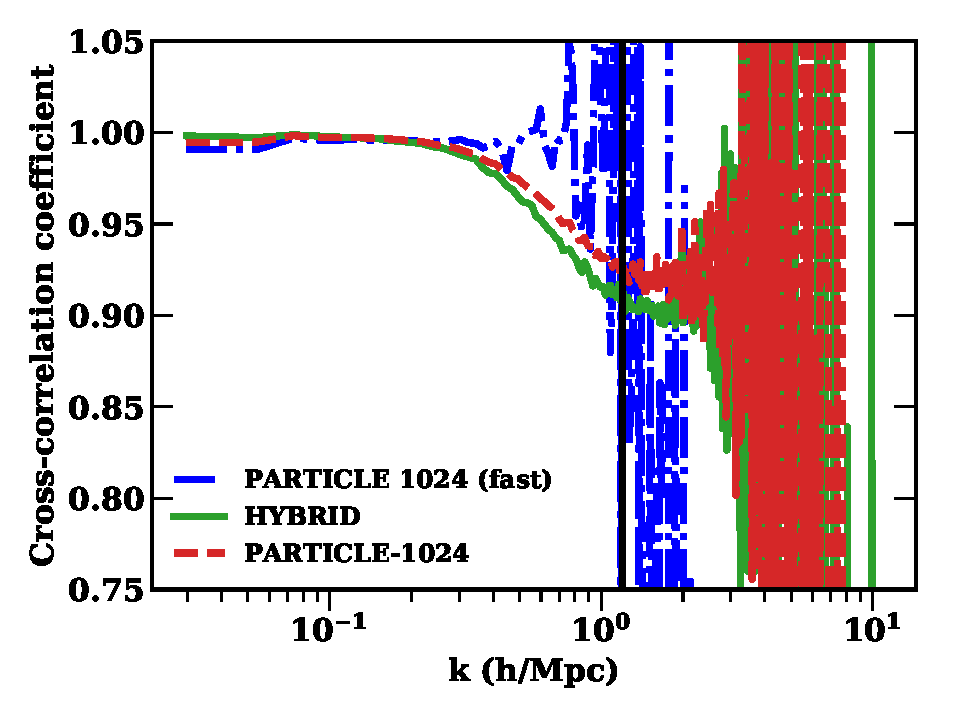
\includegraphics[width=0.45\textwidth]{nuplots/corr_coeff-1.pdf}
  \caption{The cross-correlation coefficient between neutrinos and dark matter using the particle and hybrid simulation methods.
  The cross-correlation is unity for scales where the neutrino power is not dominated by shot noise (vertical dotted line), justifying the use of
  this approximation in the linear response method.
  }
  \label{fig:cross-corr}
\end{figure}

In this section we describe the semi-analytic linear response method for treating neutrinos from \cite{AHB}.
Motivated by the numerical difficulties with particle simulations, we sought to use an analytic treatment.
The applicability of this method follows is because neutrinos do not cluster below their free-streaming length, given by
\begin{equation}
 k_{\rm fs}(z) \approx \frac{0.08}{\sqrt{1+z}}
\sqrt{\frac{\Omega_{\rm M}}{0.3}} \frac{m_{\nu}}{0.1 ~ \textrm{eV}} h~ \textrm{Mpc}^{-1}.
\label{eq:kfs}
\end{equation}
For astrophysically relevant neutrino masses, this free-streaming length is larger than the non-linear scale.
Thus while cold dark matter exhibits strong non-linear clustering, the neutrino species does not, behaving
almost as expected from linear perturbation theory. However, the neutrino species does exhibit increased clustering
as a result of the deeper non-linear cold dark matter potential. The method of \cite{AHB} is thus a linear response,
in which the neutrino linear theory perturbation grows due as a result of the non-linear growth in the cold dark matter potential.

The neutrino power-spectrum is then given by (eq. (63) of \cite{AHB})
\begin{align}
P_{\nu}^{1/2}(k, \tau) &= \mathcal{I}_{s_i, s}
P_{\nu}^{1/2}(k, \tau_i) \left\{1 - (s - s_i)  a_i [\theta_{\nu}/\delta_{\nu}]_{i}(k)\right\}\nonumber\\
&+ \frac32 \Omega_{\rm M} H_0^2 \int_{\tau_i}^{\tau} \mathcal{I}_{s', s}
P^{1/2}_{\rm M}(k, \tau') (s - s')d \tau', \label{eq:P-final}
\end{align}
where $\mathcal{I}_{s_1, s_2} \equiv \mathcal{I}([s_2 -s_1]k/m)$. $\mathcal{I}$ is defined to be
the Fourier transform of the unperturbed neutrino distribution function in momentum space, normalized so
that $\mathcal{I}(0) = 1$ \citep{Brandenberger_1987, Bertschinger_Watts_1988},
\begin{equation}
\mathcal{I}[X; f_0] \equiv \frac{\int dq~ j_0(q X) q^2 f_0(q) }{\int dq ~q^2 f_0(q)}. \label{eq:I.def}
\end{equation}

The first term of Eq.~\ref{eq:P-final} represents a contribution from the initial conditions. In practice
for astrophysical masses neutrinos are initially relativistic, so this term is extremely small and may
be safely neglected (although we include it in our implementation for completeness).
The second term is the perturbation to a neutrino geodesic from the CDM potential
integrated over cosmic time. Our implementation computes the matter power spectrum for every PM timestep
and stores it in a table, evenly spaced in $\Delta a = 0.01$\footnote{The code actually provides the CDM power spectrum.
We estimate the matter power spectrum by adding the neutrino power from the previous timestep. It would be possible
to iterate this procedure, but in practice it is always immediately converged to a high degree of accuracy.}.
The neutrino power spectrum is computed by performing an integral over all past matter power spectra, interpolated in log space.

Eq.~\ref{eq:P-final} computes the neutrino power spectrum from stored CDM power spectra.
A computation of the neutrino potential would use the CDM potential over all of cosmic history, which is impractical
to store at the required number of time slices. We make the approximation that neutrinos and
have a cross-correlation coefficient of unity. Thus, in order to recover the neutrino potential, we use
\begin{equation}
\delta_{\nu}(\bs k, \tau) = \left(\frac{P_{\nu}(k,
    \tau)}{P_{\rm cdm}(k, \tau)}\right)^{1/2} \delta_{\rm cdm}(\bs k, \tau).\label{eq:phases}
\end{equation}
Equivalently, we assume that the neutrinos and CDM have identical Fourier phases or that neutrinos perfectly trace CDM structure.
Physically, this is plausible: neutrinos behave much like CDM on scales larger than their free streaming length,
and do not cluster on smaller scales (so any differences in their phases has limited practical impact, as $\delta_\nu$ is zero).
Figure~\ref{fig:cross-corr} shows the cross-correlation coefficient,
\begin{equation}
R = \frac{\left\langle \delta_\nu \delta_\mathrm{cdm} \right\rangle}{\sqrt{P_{\rm{cdm}} P_{\rm{\nu}}}}
\end{equation}
between neutrinos and CDM from a neutrino particle simulation. It is indeed unity on large scales,
dropping to zero on small scales where the particle neutrino power is dominated by shot noise.

\subsection{Hybrid Neutrinos}
\label{sec:hybrid}

\begin{figure}
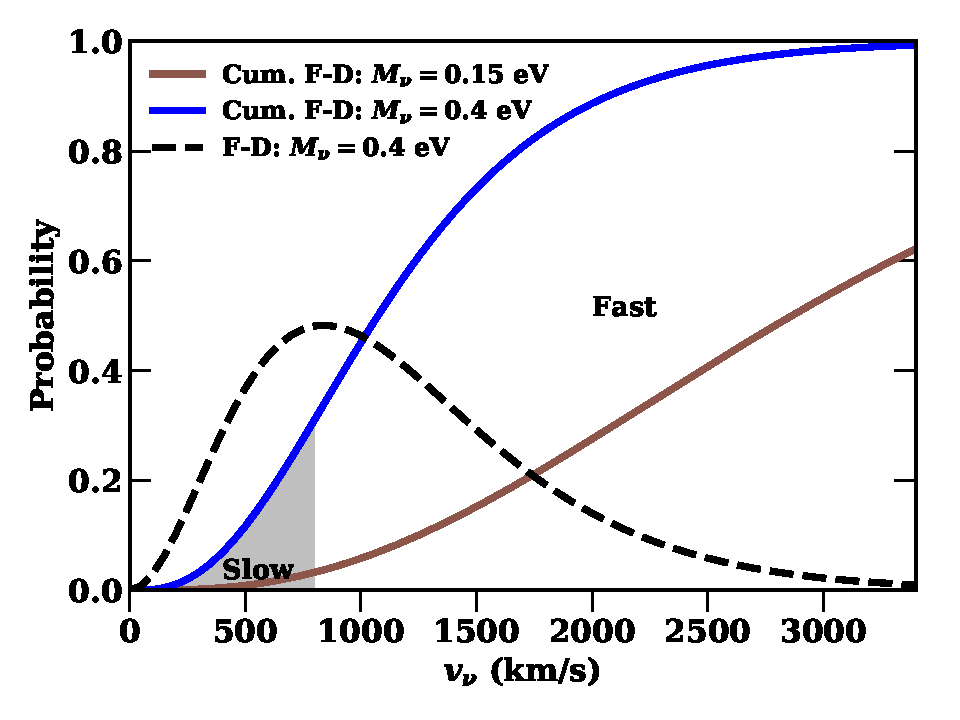
\includegraphics[width=0.45\textwidth]{nuplots/fermidirac.pdf}
  \caption{The integrated Fermi-Dirac distribution, showing the cumulative probability for neutrinos to have an unperturbed velocity less than $v_\nu$ at $z=0$ for total neutrino mass $M_\nu = 0.4$ eV.
  The grey shaded region shows the neutrino density followed by particles in our hybrid method.
  }
  \label{fig:fddistribution}
\end{figure}

\cite{AHB} showed that the linear response neutrino simulation method did not fully reproduce the neutrino power spectrum on small scales. This initially appears strange; we showed that the neutrino free-streaming length is larger than the non-linear scale, so how do neutrinos cluster non-linearly? The answer is that the initial thermal velocity of neutrinos is not a delta function, but a Fermi-Dirac distribution. Neutrinos drawn from the slow tail of the distribution will have a smaller free-streaming length, whch may be smaller than the non-linear scale. Such slow neutrinos make up a small fraction of the total matter density, but can still dominate the power spectrum because the clustering of faster neutrinos is heavily suppressed.

Building on this insight, we have implemented a hybrid particle-linear response neutrino simulation method. Neutrinos are split into fast and slow components, based on their Fermi-Dirac velocities. Figure~\ref{fig:fddistribution} shows the cumulative Fermi-Dirac distribution graphically, with the shaded area under the curve indicating the slow neutrino component. When generating initial conditions for the simulation, we create N-body particles with thermal velocities matching the (redshifted) slow neutrino component.\footnote{Our hybrid method differs substantially from the similarly named technique described in \cite{Brandbyge_2010}. In that work, neutrino particles are dynamically created during the simulation, when neutrino clustering exceeds a threshold. In our implementation, the neutrino particles generated with the initial conditions, but do not gravitate initially.}

Initially these ``slow neutrino'' N-body particles behave as tracers; they experience gravitational force from the cold dark matter, but they do not gravitate. The neutrino component is followed entirely by the linear response method described 
in Section~\ref{sec:analytic}. Our hybrid method thus avoids being affected by neutrino shot noise or early-time relativistic effects.

Slow-moving neutrinos are distributed completely homogeneously in the simulation initial conditions. The velocities expected from structure formation at the initial redshift are substantially smaller than neutrino thermal velocities, even for slow neutrinos. 
We verified explicitly that our results at all redshifts were unchanged for a simulation where our slow-moving neutrinos had an initial clustering matching the transfer function of the cold dark matter, a conservative over-estimate of the true initial clustering.

Once the simulation reaches a critical redshift, the particle neutrinos are ``switched on'' and begin to gravitate.
After this point the linear response method is modified to reduce the matter density in the analytic neutrino component by the amount of mass in the neutrino particles. We also modify the neutrino power spectrum calculation so that neutrino perturbations are included only for unperturbed velocities faster than those sampled by the ``slow-moving'' neutrino particles. 
In other words \spb{TODO: YAH analytic formula from YAH here}.

We use the following asymptotic expansion for the integral:
\begin{align}
 \int^\infty_{q_\mathrm{c}} \frac{j_0(qX) q^2}{e^q + 1} q^2 dq &= - \Sigma^{\infty}_{n=1} (-1)^n \frac{\exp^{-n q_\mathrm{c}}}{(n^2+X^2)^2} I_n(q_\mathrm{c},X) \;,\\
 I_n(q_\mathrm{c},X) &= (n^2 + n^3 q_\mathrm{c} + n q_\mathrm{c} X^2 - X^2) \frac{\sin(q_\mathrm{c} X)}{X} \\
 &+ (2n + n^2 q_\mathrm{c} + q_\mathrm{c} X^2) \cos(q_\mathrm{c} X)\;,\\
\end{align}
which we have confirmed, using mathematica, to be accurate to $0.1\%$.
\spb{End analytic results from YAH}.

By default we consider the ``slow-moving '' tail of the Fermi-Dirac distribution to be all neutrino density with an unperturbed velocity less than $750$ (comoving) km/s. We found by experiment that this value was the smallest that led to good agreement 
with the particle neutrino method. The effects of other cutoff velocities are discussed in Section~\ref{sec:results}.
The critical redshift at which particle neutrinos switched on was set at $z=1$, for similar reasons.

Our hybrid neutrino implementation does not include the neutrino hierarchy, assuming all three neutrino species are degenerate. The inclusion of the neutrino hierarchy in future work should not be difficult, but we deferred it because the masses where it is important ($M_\nu < 0.15$~eV) are sufficiently low that their clustering is already adequately modelled by our linear response method.

Note that our hybrid neutrino technique still imposes some numerical overhead above the linear response method, because of the need to evolve the tracer neutrinos with small timesteps at early times. We attempted to avoid this by inserting neutrinos dynamically at a late time, but accurately modelling the non-linear distortions to the analytic Fermi-Dirac function proved overly complex. The overhead is reduced from purely particle neutrino simulations, both because fewer neutrino particles are needed to achieve a given level of shot noise and because the particle neutrinos are moving more slowly. However, since there is still some overhead, we recommend that simulators which do not require high accuracy in the neutrino power spectrum use the linear response method.

\subsection{Simulations}
\label{sec:simulations}

Our simulations were run with MP-Gadget \url{https://github.com/rainwoodman/MP-Gadget/} and are detailed in Table \ref{tab:simulations}. We used a box size of $300$ comoving Mpc/h with $512^3$ cold dark matter particles,
initialised using a CDM+baryon transfer function at $z=99$. Each simulation has the same initial phases,
ensuring the same distribution of late-time halos. We have performed simulations with massless neutrinos, and a linear response simulation with the minimal neutrino mass allowed by oscillation experiments, $M_\nu = 0.06$ eV (and a normal neutrino hierarchy). All other simulations have a total neutrino mass of $0.4$~eV, and assume a degenerate neutrino hierarchy. We used a relatively high neutrino mass $0.4$~eV was chosen because it is the minimal neutrino mass for which the linear response method fails to accurately reproduce the neutrino power spectrum on these scales.

We have performed three simulations which differ only in the neutrino simulation method; one with linear response, one with particle neutrinos and one with our new hybrid implementation. We then performed a number of simulations designed to test the sensitivity of our hybrid method to numerical parameters. Our default hybrid neutrino simulation uses a critical velocity of $750$ (comoving) km/s, a neutrino switch-on time of $z_\nu = 1$ and includes $512^3$ neutrino particles, matching the cold dark matter. Our modified simulations included one with a neutrino switch-on time of $z_\nu = 4$, one with $256^3$ neutrino particles, and simulations with critical velocities of $1000$ and $5000$ km/s. The simulation with a critical velocity of $5000$ km/s includes all the neutrino power in particles after the neutrino switch-on time and is thus useful as a comparison to the pure particle method. We finally performed a simulation with a critical velocity of $500$ km/s, verifying that this was too small to achieve a converged neutrino power spectrum.
For reference, the fraction of the neutrino matter density in particles for critical velocities of $500$, $750$, $1000$, $5000$ (comoving) km/s is $0.117$, $0.276$, $0.451$ and $1$ respectively.

%TABLE OF SIMULATIONS.
\begin{table}
\begin{center}
\begin{tabular}{|l|c|c|c|c|l|}
\hline
% Name & $M_\nu$ (eV) & Method & Box (Mpc/h) & $N_\mathrm{part}^{1/3}$ & Notes \\
% \hline
%     &       0             &    -          & 512         & 512       &       \\
%     &       0             &    -          & 300         & 512       &       \\
%     &     0.4             &   Analytic    & 300         & 512       &       \\
%     &     0.4             &   Particle    & 300         & 512       &       \\
%     &     0.4             &   Hybrid      & 300         & 512       &  $256^3$ nu particles    \\
%     &     0.4             &   Hybrid      & 300         & 512       &  $256^3$ nu particles    \\
%     &     0.4             &   Hybrid      & 300         & 512       &  $256^3$ nu particles    \\
%     &     0.4             &   Hybrid      & 300         & 512       &  $256^3$ nu particles    \\
%     &     0.4             &   Hybrid      & 300         & 512       &  $256^3$ nu particles    \\
    Name & $M_\nu$ (eV) & Method & $N_\mathrm{nu}^{1/3}$ & $v_\mathrm{crit}$ & Notes \\
\hline
CDM    &       0             &    -          & 0         & - &    \\
MINNU    &     0.06            &   Analytic    & 0         & - &  Normal hier.  \\
LINRESP    &     0.4             &   Analytic    & 0         & - &    \\
PARTICLE    &     0.4             &   Particle    & 512       & - &    \\
%     &     0.4             &   Hybrid      & 256     &   &    \\
HYBRID    &     0.4             &   Hybrid      & 512       & 750 & \\
HYBSING    &     0.4             &   Hybrid      & 256       & 750 & \\
VCRIT    &     0.4             &   Hybrid      & 512       & 1000 & \\
HYBALL    &     0.4             &   Hybrid      & 512       & 5000 & $z_\nu = 4$ \\
NUTIME    &     0.4             &   Hybrid      & 512       & 5000 & $z_\nu = 1$  \\
%    &     0.4             &   Hybrid      & 512       & 500 &    \\

\hline
\end{tabular}
\end{center}
\caption{Table of simulation parameters. All simulations have a box of $300$ Mpc/h
and $512^3$ cold dark matter particles.
}
\label{tab:simulations}
\end{table}

% Mnu = 0  (300)

% Mnu = 0.4: analytic, particle, hybrid. (300)
%
% Checks (all Mnu=0.4, hybrid, (300)):
% Varying vcrit from 500 to 300
% Varying NuPartTime from 0.333 to 0.5
% Number of hybrid particles from 256 to 512.
% Mnu = 0.06: analytic (300, 512)

%Todo:
%(300,512,1024 *neutrinos* for hybrid?)

\section{Results}
\label{sec:results}

\begin{figure*}
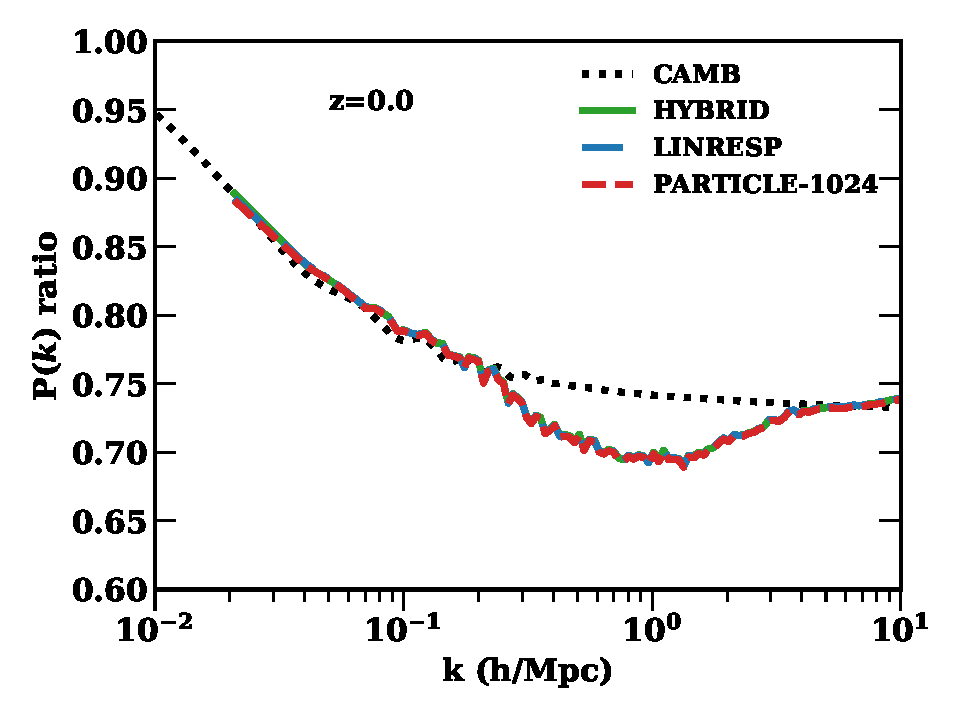
\includegraphics[width=0.45\textwidth]{nuplots/pks_rel-10.pdf}
\includegraphics[width=0.45\textwidth]{nuplots/pks_rel-0_83330.pdf}
  \caption{Plot showing the matter power spectrum ratios between analytic, particle and hybrid methods at (Left) $z=0$ and (Right) $z=0.2$. Note the slightly reduced power in the particle method - this is a consequence of the inability to correctly treat the time-varying mass of neutrinos.
  }
  \label{fig:matter_power}
\end{figure*}

\begin{figure}
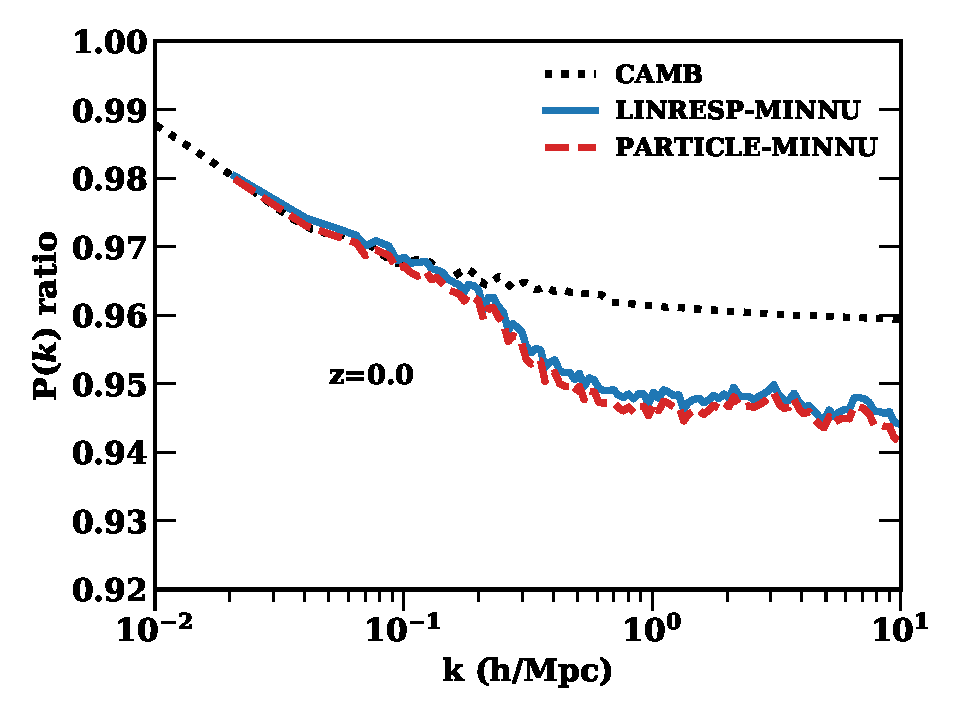
\includegraphics[width=0.45\textwidth]{nuplots/pks_lowmass-10.pdf}
\caption{Plot showing the matter power spectrum ratio at $z=0$ between massless neutrinos and minimal neutrino mass; one massive neutrino with a mass of $0.06$ eV.
}
\label{fig:minimal_mass}
\end{figure}

\begin{figure*}
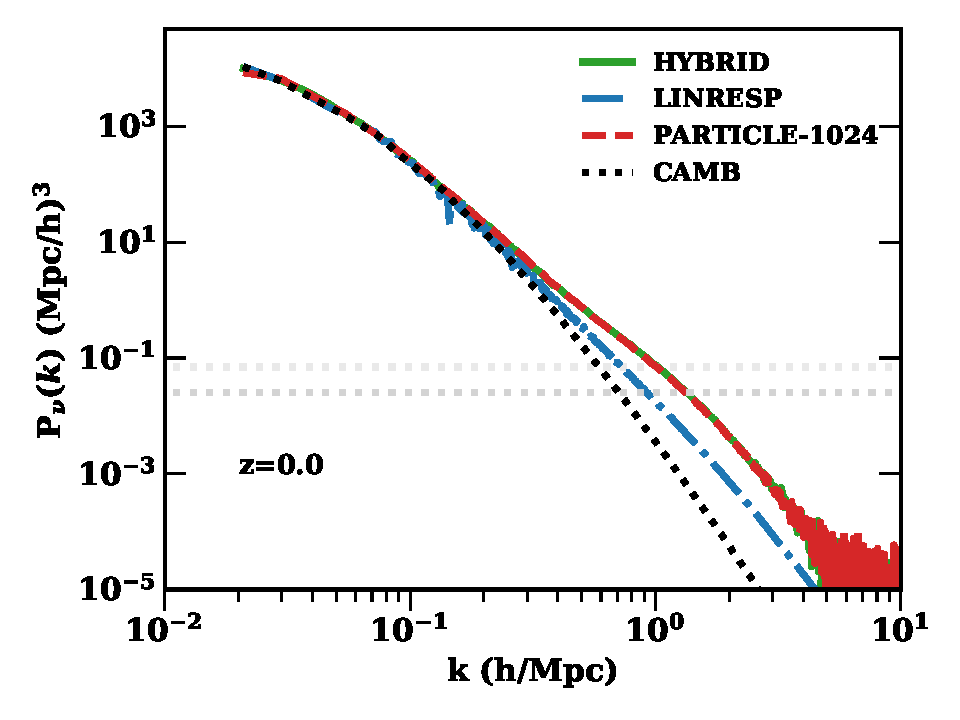
\includegraphics[width=0.45\textwidth]{nuplots/pks-nu-1.pdf}
\includegraphics[width=0.45\textwidth]{nuplots/pks-nu-0_8333.pdf}
  \caption{Plot showing the neutrino power spectrum ratios between particle, analytic and hybrid.
  (Left) At $z=0$. (Right) At $z=0.2$.
  MONEY PLOT.}
  \label{fig:neutrino_power}
\end{figure*}

\begin{figure*}
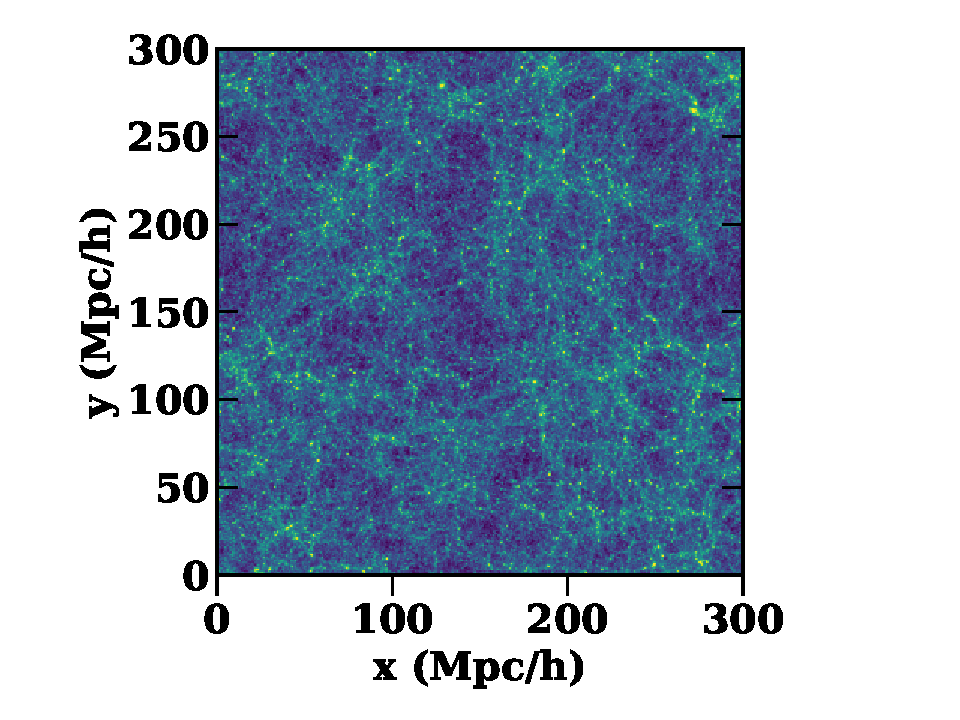
\includegraphics[width=0.3\textwidth]{nuplots/dens-plt-b300p512nu0_4hybt1.pdf}
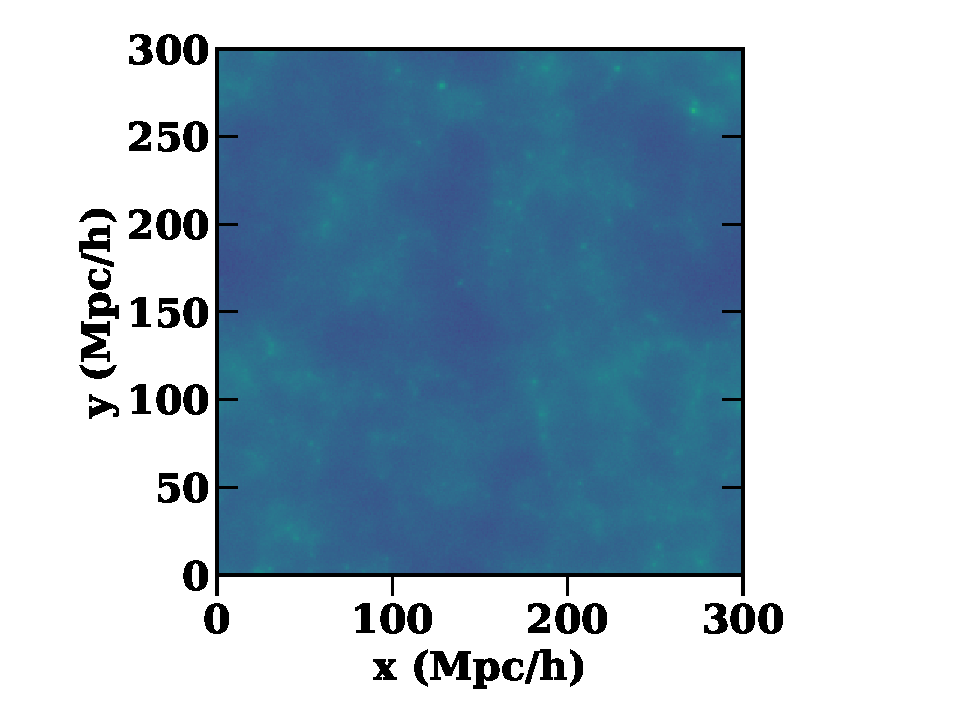
\includegraphics[width=0.3\textwidth]{nuplots/dens-plt-b300p512nu0_4hybt2.pdf}
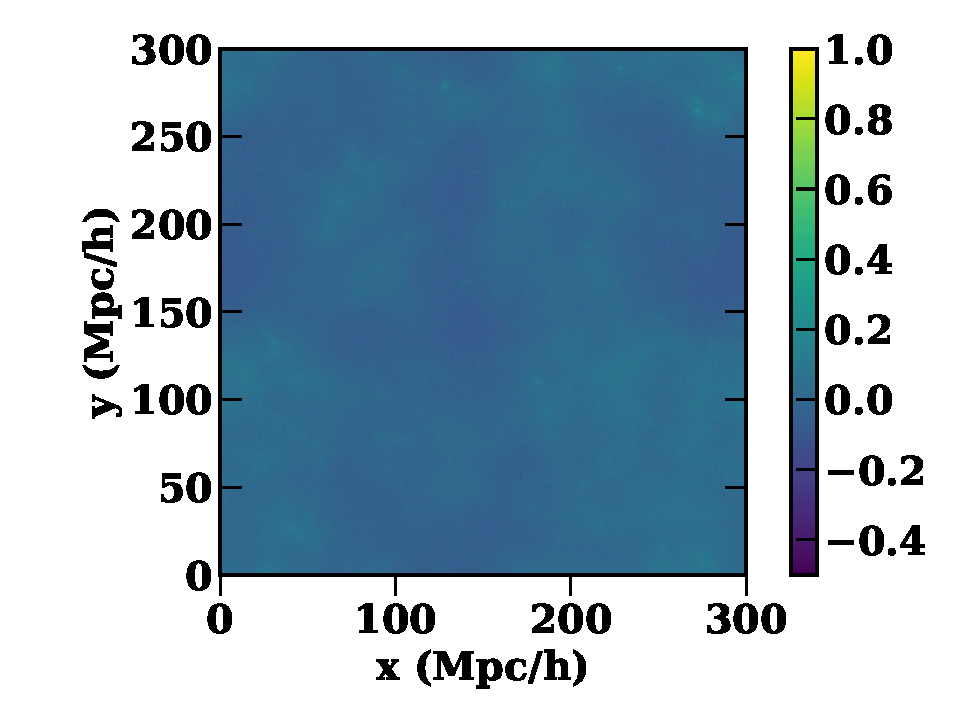
\includegraphics[width=0.3\textwidth]{nuplots/dens-plt-b300p512nu0_4pt2.pdf}
  \caption{Projected density plots at $z=0$. (Left) Cold dark matter. (Middle) Neutrino particles from the hybrid simulation, with initial velocity $<750$ (comoving) km/s. (Right) Neutrino particles from the pure particle simulation. No correction has been made for shot noise. The clustering of the hybrid particles is intermediate between that of the cold dark matter and the particle neutrinos. Notice how the positions of clusters and voids is the same in all three panels.}
  \label{fig:density_plot}
\end{figure*}

In this Section we show the results of our simulations at low redshift for all three methods: particle, linear response and hybrid. Figure~\ref{fig:matter_power} shows the ratio of the matter power spectrum for our three methods at $z=0$ and $z = 0.2$ to the matter power spectrum of the massless neutrino CDM simulation. The HYBRID and LINRESP simulations are indistinguishable, differing by around $0.1\%$. The PARTICLE simulation shows a reduction in power of about $1-2\%$. This deficit is because the particle simulation does not include the increased mass of the neutrinos at early times, when they are relativistic, and thus slightly underestimates $\Omega_M$ between $z=99$ and $z=49$.\footnote{Note this discrepancy did not appear in \cite{AHB} because of the slightly inaccurate initial conditions detailed in Appendix \ref{sec:initcond}, which masked it by neglecting relativistic effects in all methods.}
The effect of neutrinos differs from the linear theory, as calculated by CAMB, at $k \sim 0.2$ Mpc/h.
Figure \ref{fig:minimal_mass} shows the results of the $M_\nu = 0.06$~eV linear response simulation at $z=0$, demonstrating that this simulation differs from linear theory at a similar scale, and further demonstrating that our simulations are converged and now able to reproduce the results of linear theory on large scales even for the lowest neutrino mass allowed by oscillation experiments, a feat never possible with particle neutrinos.

Figure~\ref{fig:neutrino_power} compares the power spectrum of the neutrinos in each of our methods, as well as the linear theory power spectrum, at $z=0$ and $z=0.2$. For the HYBRID simulation we have computed the total neutrino power spectrum as the weighted sum of the power spectrum of the fast and slow components $P^{1/2}_\nu = f_\mathrm{fast} P^{1/2}_\mathrm{fast} + f_\mathrm{slow} P^{1/2}_\mathrm{slow}$, where $f_\mathrm{fast} + f_\mathrm{slow} = 1$.
We have subtracted shot noise at the level shown in the Figure. Remarkably the neutrino power appears recoverable even two orders of magnitude below the shot noise level. Note that the shot noise for the HYBRID simulation is a factor of three lower than for the PARTICLE simulation, as the matter density in particle neutrinos is only one third of the total neutrino density. The neutrino power spectrum in the PARTICLE and HYBRID simulations agree by eye extremely well \spb{Lower panel with ratios?}, doubly remarkable given that the PARTICLE method does not reproduce the total matter clustering. Both methods show sharply increased neutrino power on small scales over the linear response method. We verified that at $z=1$ all three methods were in reasonable agreement.
It thus seems that the hybrid method indeed improves agreement for the neutrino power spectrum.

In order to give a visual impression of the clustering of the neutrinos and dark matter, Figure \ref{fig:density_plot} shows projected densities for the CDM next to neutrino particles from the HYBRID and PARTICLE simulations.\footnote{Projected density plots made using Nbodykit.} It is visually apparent that the structure of filaments, halos and voids is identical in all three plots, further reinforcing the conclusion of Figure \ref{fig:cross-corr} that the phases of the neutrinos and CDM are highly correlated. The increased clustering of the hybrid neutrinos, drawn from the initially slower part of the Fermi-Dirac distribution, is also apparent when compared to the particle neutrinos. However, they still cluster less than the CDM.

\subsection{Numerical Checks}

\begin{figure*}
  \includegraphics[width=0.45\textwidth]{nuplots/pks-cknu-1.pdf}
  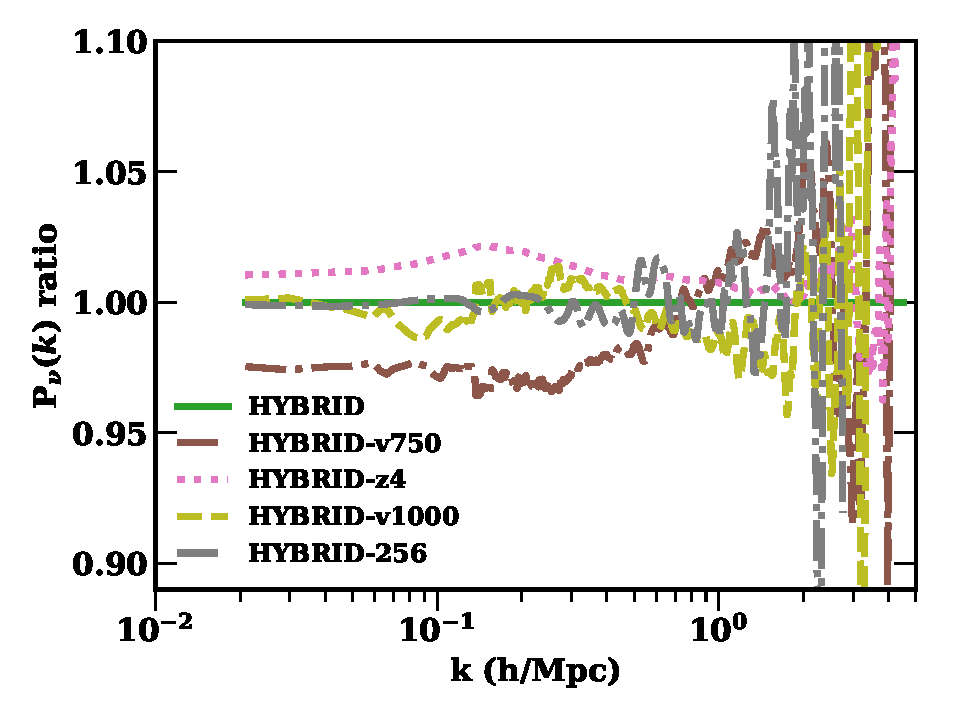
\includegraphics[width=0.45\textwidth]{nuplots/pks_nu_ckrel-1.pdf}
  \caption{Plot showing the neutrino power spectrum from our numerical checks, at $z=0$. We have varied the neutrino switch-on time, the critical neutrino velocity and the number of neutrino particles. (Left) Absolute neutrino power spectrum. (Right) Ratio of neutrino power spectra to the HYBALL simulation. We have subtracted the neutrino shot noise in all cases. Note that to reduce mode-to-mode scattering, the ratio curves have been smoothed.}
  \label{fig:vcrit}
\end{figure*}

% \begin{figure}
%     \includegraphics[width=0.45\textwidth]{nuplots/P_nu_M500_z0.pdf}
%     \caption{Plot showing CDM simulation with test particle neutrinos with fixed (not FD) single velocity of $500$ km/s at $z=0$. Neutrino power spectrum, compared to analytic $P_{CDM}$.\spb{I can't find the analytic estimates anymore...need to reproduce them. Also not sure I trust these specific simulations: I found some gadget bugs along the way. They should be re-run or possibly removed.}}
%    \label{fig:testpart}
% \end{figure}
%
Figure~\ref{fig:vcrit} shows the effects of changing various numerical parameters of our hybrid neutrino simulations. All simulations agree to within $10\%$ until $k = 2$ Mpc/h, which corresponds to the mean inter-particle spacing of the simulation. We consider this an acceptable degree of convergence for a quantity which is less than $1\%$ of the total matter density. In particular the PARTICLE and HYBALL simulations agree extremely well: these two simulations differ only in their treatment of neutrinos at $z > 4$. The PARTICLE simulation shows about $2\%$ less power than the HYBALL simulation, a similar deficit to the differences in the total matter power spectrum. The NUTIME simulation is identical to HYBALL, except that the neutrino switch-on time is $z=1$. This simulation has a power deficit of about $5\%$ on large scales. Note that it is likely the result of the NUTIME simulation is preferable; at high redshift the neutrino component suffers from shot noise, which may be leading to artificial structure growth in the neutrinos. Alternatively, there may be some genuine real structure growth which is being missed, although this seems unlikely at these large scales.

The ratio with simulations which alter the neutrino critical velocity are somewhat noisy, an unfortunate consequence of combining the analytic and particle neutrino power spectra, which have slightly different mode-to-mode scatters. When all neutrinos are particles, this mode-to-mode scatter is the same for both simulations and disappears in the ratio. This scatter should be understood as a consequence of the finite accuracy of the Gadget gravity solver when dealing with a particle component making up less than $1\%$ of the total matter density. The VCRIT simulation, which also has a neutrino switch-on time of $z=1$, agrees well with the NUTIME simulation. The increased power around $k \sim 1$ is likely a consequence of the increased effective resolution in the neutrino component and thus slightly increased non-linear growth. The few percent changes at large scales are probably noise. The HYBRID simulation, with a slightly smaller critical velocity of $750$ km/s, exhibits $0-5\%$ less power at $k=0.1 - 0.5$ h/Mpc. While this could also be due to shot noise, we suspect this is because this simulation misses some real non-linear structure formation on these scales. We performed another simulation with a neutrino critical velocity of $500$ km/s, and found a similar, but larger, reduction in power. Furthermore, the HYBSING simulation, which is identical to HYBRID but with $8$ times fewer particles, gives identical results to the HYBRID simulation, suggesting that shot noise is not having a large effect. This is somewhat remarkable, given that at $k=2$ and $z=0$ shot noise dominates by a full order of magnitude, and it suggests that future users of this simulation code may use reduced particle numbers with confidence. Similar results are seen at other redshifts, although convergence is markedly worse ($20-30\%$) at the neutrino switch-on time in all cases.

\section{Conclusions}
\label{sec:conclusion}

We have extended our semi-analytic linear response neutrino simulation method from \cite{AHB} to include hybrid neutrinos, where a fraction of the neutrino density, drawn from the slow part of the Fermi-Dirac distribution, is followed by neutrino particles at late times. With this modification we show that we can reproduce the neutrino power spectra of well-converged particle methods and the large-scale total matter power expected by linear theory and predicted by the linear response method. We recommend that those wishing to compare observational surveys to simulations use the semi-analytic linear response method, as that reproduces all directly observable quantities, in particular the total matter power spectrum, galaxy clusters \citep{McCarthy_2017}, the weak lensing shear \citep{Liu_2017} and the Lyman-alpha forest \citep{AHB}. To aid this we have helpfully provided this method as a patch to Gadget-2 as well as integrated it into the public code MP-Gadget. The linear response code is computationally very efficient, involving a single integration for every PM timestep, and we have attempted to ensure that it will be easy to integrate into any structure formation code.

For simulators wishing instead to investigate the structure of the neutrino component of matter around collapsed objects \citep{FVN_2013}, neutrino wakes \cite{Inman_2015} or other explicitly non-linear objects, we recommend using the full hybrid neutrino code. For example, in future work one could compute the neutrino bispectrum \citep{Furhrer_2015} or use our method to examine the distribution of massive neutrinos in cosmic voids, which \cite{Banerjee_2016} argued would not be correctly followed by our linear response method. We suggest a neutrino switch-on redshift $z=1$ and a critical neutrino velocity of $750-1000$ km/s, which gave the best results in our tests. We further suggest that most simulators use a mean interparticle spacing for the neutrino component double that for the CDM, and thus $1/8$th the number density, as this gave identical results in our tests with much smaller computational overhead.

Finally, we note that cosmological surveys have now reached a level of sensitivity where even the minimal neutrino mass can substantially alter derived parameters \cite{Calabrese_2017}, and thus the inclusion of massive neutrinos (and radiation in the background) should become standard for all simulators.

\section*{Acknowledgements}

This research project (or part of this research project) was conducted using computational resources (and/or scientific computing services) at the Maryland Advanced Research Computing Center (MARCC).
SB was supported by NASA through Einstein Postdoctoral Fellowship Award Number PF5-160133.

\appendix

\section{Manual}
\label{sec:manual}

In this Appendix, we briefly describe the parameters of the linear response neutrino method. A similar description may be found in the README of the code repository: \url{https://github.com/sbird/kspace-neutrinos/}. Our neutrino integrator has been altered to be a stand-alone module, largely independent of the underlying N-body code. To aid integration, we have included copious comments and unit tests. A script is provided in the repository which downloads and patches a fresh copy of Gadget-2 to include massive neutrinos: the ``apply-patches'' script in the gadget-2 subdirectory.

Table \ref{tab:parameters} shows a list of the required parameters, as well as brief descriptions. The number of extra parameters required is small. Three parameters are required to specify the initial power of the neutrino component, using a CAMB or CLASS transfer function file. Three parameters are required to specify the masses of the three active neutrino species. Finally, three parameters are used for the properties of the hybrid neutrino model: a global switch enabling the model, the critical velocity below which neutrinos are particles, and the neutrino switch-on time, after which neutrinos are actively gravitating.

%TABLE OF SIMULATIONS.
\begin{table*}
\begin{center}
\begin{tabular}{|l|l|}
\hline
    Parameter & Description \\
\hline
KspaceTransferFunction   & CMB transfer functions, used to compute the neutrino the neutrino integration. \\
TimeTransfer             & Scale factor of the CMB transfer functions. \\
InputSpectrumUnitLengthincm   & Units of the CAMB transfer function in cm. \\
MNue, MNum, MNut &  Three neutrino masses. For full generality, no neutrino  hierarchy is enforced. \\
Vcrit            & Critical velocity below which the neutrinos are particles, if hybrid neutrinos are on. \\
NuPartTime       & Scale factor at which the particle neutrinos start to gravitate, if hybrid neutrinos are on. \\
HybridNeutrinosOn       & Switch to enable hybrid neutrinos. \\
\hline
\end{tabular}
\end{center}
\caption{Table of code parameters, with brief descriptions.}
\label{tab:parameters}
\end{table*}

As documented in \cite{Springel_2005} and the Gadget-2 manual, all versions of Gadget output snapshots mid-timestep. This is implemented by drifting all particles (even those not currently active) to the desired output time. However, particles are not kicked to update their momenta, so that the output particle velocities are those from the last active timestep. For neutrino particles, whose clustering is intimately tied to their total momentum, restarting from a snapshot using Gadget-2 or later will introduce an error in the $z=0$ power spectrum. We therefore strongly recommend that Gadget-2 simulators restart their simulations, if necessary, from restart files. This does not apply for MP-Gadget, which we have modified so that snapshots always occur at the end of a PM timestep, when all particles are active.

\section{Initial Conditions}
\label{sec:initcond}

\begin{figure*}
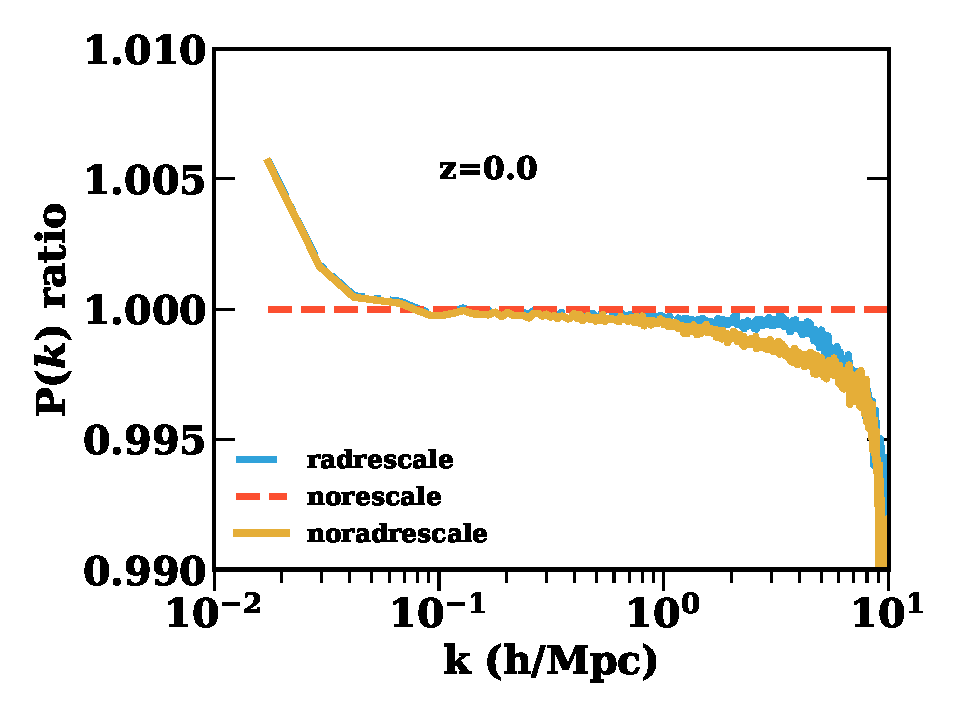
\includegraphics[width=0.45\textwidth]{icplots/pks_rel-1.pdf}
\includegraphics[width=0.45\textwidth]{icplots/pks_camb-1.pdf}
  \caption{(Left) The $z=0$ power spectrum from three simulations.
  These are initialised respectively with the $z=99$ transfer function,
  the scaled $z=0$ transfer function, and the $z=0$ transfer function
  scaled and evolved neglecting radiation density.
  Curves are normalised to the simulation using the scaled $z=0$ transfer function.
  (Right) The same three simulations normalised to the linear matter
  power spectrum from CAMB at $z=0$.}
  \label{fig:rescaling0}
\end{figure*}

\begin{figure*}
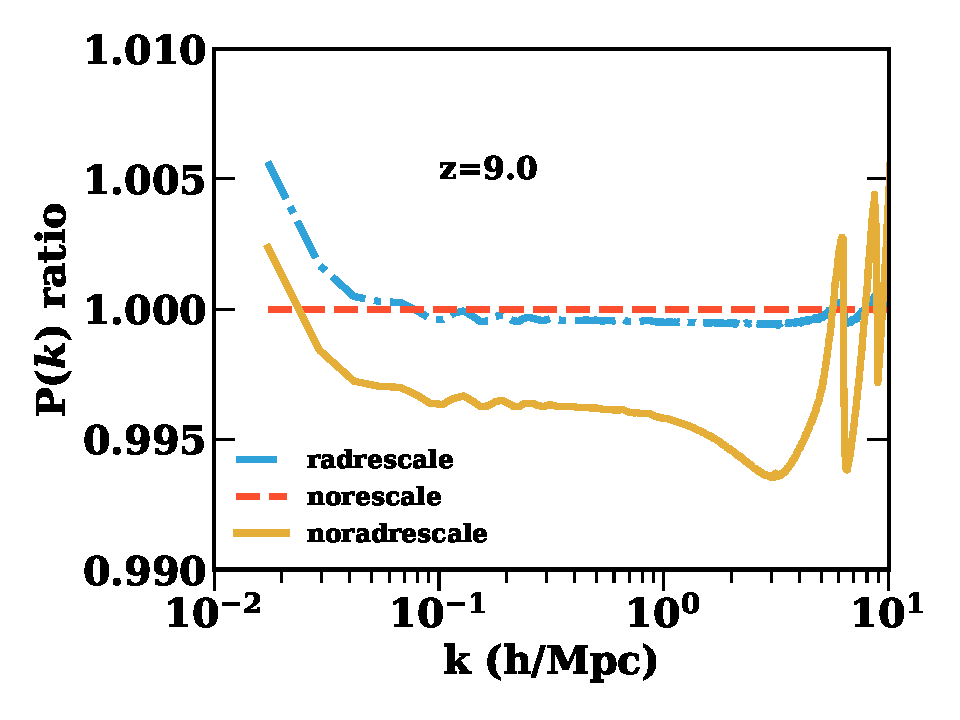
\includegraphics[width=0.45\textwidth]{icplots/pks_rel-0_1.pdf}
\includegraphics[width=0.45\textwidth]{icplots/pks_camb-0_1.pdf}
  \caption{(Left) The $z=10$ power spectrum from three simulations.
  These are initialised respectively with the $z=99$ transfer function,
  the scaled $z=0$ transfer function, and the $z=0$ transfer function
  scaled and evolved neglecting radiation density.
  Curves are normalised to the simulation using the scaled $z=0$ transfer function.
  (Right) The same three simulations normalised to the linear matter
  power spectrum from CAMB at $z=0$.}
  \label{fig:rescaling10}
\end{figure*}

%Show higher redshift?

Since \cite{AHB}, we have improved our initial conditions, generated
using our freely available initial conditions code
S-GenIC \url{https://github.com/sbird/S-GenIC}. These improvements concern
the relationship between velocities and displacements in Lagrangian perturbation theory.
\citep{Zeldovich_1970, Scoccimarro_1998}. In linear Lagrangian perturbation theory,
velocities and displacements are related by a scale-independent factor

\begin{equation}
v(k) = a H(a) \frac{d \log D(a)}{d \log a} \delta(k)
\label{eq:vel_prefac}
\end{equation}
where $D(a)$ is the linear growth function and $H = \dot{a}/a$, the Hubble function.
In \cite{AHB}, the Hubble function used in Eq.~\ref{eq:vel_prefac}
neglected radiation density, leading to a small error.

Furthermore, in matter domination, the derivative of the linear growth function,
$\frac{d \log D(a)}{d \log a}$, was approximated by \citep{Bouchet:1995}
\begin{equation}
\frac{d \log D(a)}{d \log a} \approx \left(\frac{\Omega_M a^{-3}}{\Omega_M  a^{-3} + \Omega_L}\right)^{0.6}\,.
\end{equation}
However, this approximation neglects the radiation density, which becomes
non-negligible at $z > 50$. This is important particularly when considering
massive neutrinos, because at high redshift neutrinos are slightly relativistic,
and thus the background density depends slightly on the neutrino mass.

In practice these two approximations partially cancelled, leading
to results that were correct to a couple of percent. However, we
have now removed them both and use both the full Hubble function
and obtain $\frac{d \log D(a)}{d \log a}$ by numerically solving
the linear growth equation \citep{Peebles:1993}:
\begin{equation}
\frac{d}{da}\left(a^3 H(a) \frac{d D(a)}{da}\right) - \frac{3}{2} \frac{a \Omega_M}{H(a)} D(a) = 0
\end{equation}
subject to initial conditions at $z \gg 100$ corresponding
to the exact growing mode in a matter-radiation universe \citep{Groth:1975}
\begin{equation}
  D(a_i) = \Omega_r + \frac{3}{2} \Omega_M a_i\,.
\end{equation}

In the presence of baryon or neutrino fluids, the scale-independence
of the growth function is itself an approximation. For neutrinos, this
is because the free-streaming scale is redshift dependent. For baryons
it is because the baryons initially couple to the photons, suppressing
their power on scales which are sub-horizon at $z \sim 1100$. However,
by $z=99$ the baryons have already fallen into
the potential wells generated by the CDM,
and $\delta_\mathrm{b} \approx 0.7 \delta_\mathrm{CDM}$.
\cite{Zennaro_2017} showed this effect to induce only
a sub-percent error for our scales of interest and hence we neglect it.

We choose to generate our initial conditions using the CAMB total matter transfer
function at $z=99$. An alternative is to generate initial conditions
using the $z=0$ transfer function, scaled by $D(99)/D(0)$. This can
be used to account for background radiation density, if radiation is not included
in the background evolution. Even if radiation is included, it can account
for radiation perturbations and other relativistic effects on the scale
of the horizon at $z=99$ \citep{Zennaro_2017}. It also naturally accounts
for the fact that our single fluid simulations are unable to accunt for
the different growth rates experienced by baryons and CDM.

In Figure \ref{fig:rescaling0} we show the differences between the $z=0$
power spectra produced using the $z=99$ transfer function, the
scaled $z=0$ transfer function, and the $z=0$ transfer function
scaled and evolved neglecting radiation density.
For our scales of interest, these differences are slight,
especially compared to the variance induced by our finite box size.
Thus we use the $z=99$ transfer function as it is practically and conceptually simple,
whereas the linear scaling becomes complex in the presence of massive neutrinos.

Note the differences on small scales between the simulations which
include radiation in the background and the simulations which do not.
This is due to the linear growth being underestimated
at $z > 10$ in the simulations without radiation. On scales which are
already non-linear at these redshifts, non-linear growth will be inaccurately
computed. Although this effect is small, we nevertheless suggest that simulations
which use scaled $z=0$ transfer functions still include radiation in the background.
Note also that simulations with boxes $\gtrsim 2$ Gpc should somehow account
for radiation and relativistic effects.

\label{lastpage}

\bibliography{neutrinos}

\end{document}
